%subsection{Far Detector}
The main physics goal of the FD would be to measure $N_{\nu_e}(E_{\nu})$  from Formula \ref{eq:NnueEspectrum} but it would also measure $N_{\nu_\mu}(E_{\nu})$ to observe the reduced muon neutrino spectrum. Neutrinos and antineutrinos can produce signal through the CC:\\
$\nu_f+N \rightarrow f^- + N' +X$, $\bar{\nu_f}+N \rightarrow f^+ + N' +X$,\\
or through the NC:\\
$\nu_f+N \rightarrow \nu_f + N +X$, $\bar{\nu_f}+N \rightarrow \bar{\nu_f} + N +X$,\\
where f is e or $\mu$, N is a proton or a neutron, N' is another baryon, and X is other hadrons produced in the reaction.\\ \\
In case of CC, the produced charged lepton would be fully reconstructed, and also energy of all the final state particles would be summed up to reconstruct the neutrino energy. In case of NC, neutrino would not be detected, such events would be treated as a background.
The FD would be capable to efficiently reconstruct photons, electrons, muons and hadrons. \\ \\
The LBNF/DUNE FD will be located at SURF in South Dakota. There will be four modules, 10,000 tonnes of liquid argon each, placed into four caverns 1500 m underground. Each module will be 15 m wide, 12 m high and 58 m long, along the beam direction. The caverns will be placed as pairs and there will be the fifth cavern between two pairs - the one with the cryogenic equipment, to provide cooling for liquid argon.\\ \\
Key advantages of liquid argon as an FD working volume as described in \cite{ref_aboutLAr} are the ability to act as both a target and a detector, and also to operate as a tracker and a Cherenkov detector at the same time. Liquid argon is denser than water, and therefore such detector would experience more neutrino induced reactions per unit volume than a water detector would. \\ \\
The liquid argon TPC is the main working volume of the detector. The chamber is merged into the liquid argon at a temperature of 89 K. In Figure \ref{fig:farDetector_TPC}, the cathode plane assemblies (CPAs) and the anode plane assemblies (APAs) are shown. The voltages on the APAs and the CPAs are applied in such a way to create a uniform electric field between anode and cathode planes. Charged particle traveling through the electron field ionizes argon atoms. Electrons induced in the ionization process drift to the APAs and produce signal on the readout electronic elements.\\ \\
\begin{figure}
\caption{The cross section of the LArTPC for the DUNE FD (left) and the FD caverns (right). Sources of figures: \cite{ref_LBNF_CDR}}
\label{fig:farDetector_TPC}
\centering
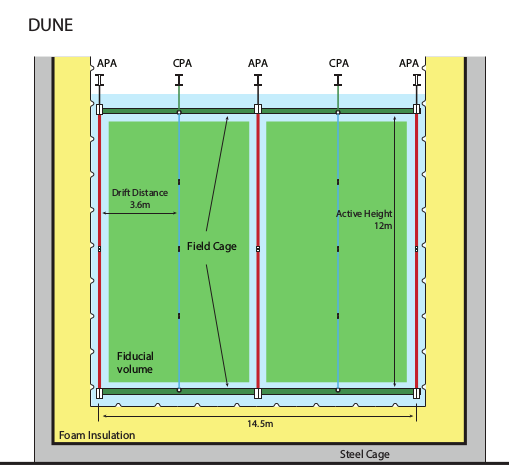
\includegraphics[width=0.5\textwidth, keepaspectratio=true]{figs/farDetector_TPC.png}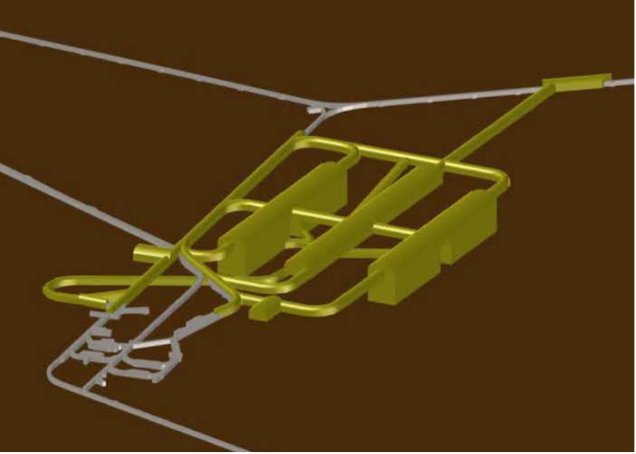
\includegraphics[width=0.5\textwidth, keepaspectratio=true]{figs/farDetector_Caverns.png}
\end{figure}
